\subsection{Sprint 1: Sockets, broadcasting and protocol definition}
In the first sprint, an early version of Tsukiji was implemented. The goal of the first sprint was to create a local simulation of the decentral market using socket connections. Messages between peers are spread via broadcasting. A basic version of the message protocol is defined. Problems encountered during this sprint are also discussed: broken pipes with disconnected sockets, identifiers, and cancel messages.

\subsubsection{Broadcasting}
Peers have to be able to communicate with each other by passing messages.
One option considered for this was approaching a subset and relaying the information of your subset to other subsets.
The issue with the subset approach was that, in a competitive market, someone that is selling an item is not easily motivated to advertise in the name of another seller.
This could lead to certain peers, that are offering an item for sale, to not relay other offers that would endanger their own offers.
This could lead to a disjoint of the network and therefor destroy communication between certain peers.
\begin{figure}[H]
  \centering
  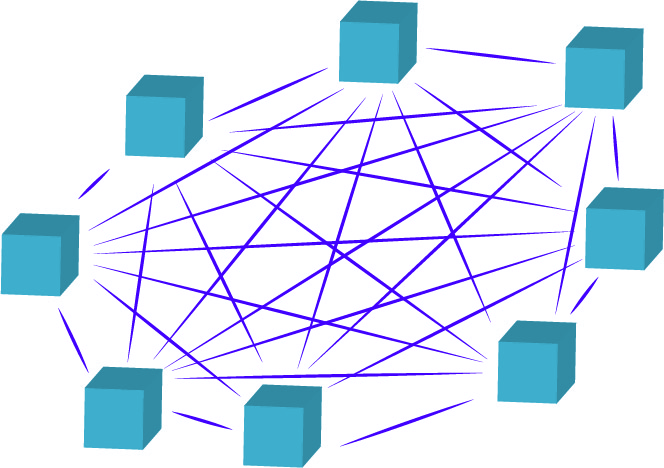
\includegraphics[width=\textwidth]{broadcasting}
  \caption{Broadcasting: The cubes represent peers and the lines represent connections between peers}
  \label{broadcastingfig}
\end{figure}

Broadcasting does not have this issue.
In broadcasting, every peer in the network is directly connected to each other, as depicted in figure \ref{broadcastingfig}.
Everyone personally takes care of their own advertising and there is no peer between origin and destination that could disrupt the communication.
The issue with broadcasting is that it scales rather poorly.
The increase of data over the network increases exponentially as the amount of users rises.
Because of this, it is not advised to use broadcasting in a large scale project.
However, broadcasting suffices for the first iteration.
Implementation is simple and it's easily replaced by a more complex system in later sprints.

\subsubsection{Protocol}
In this sprint, we also defined our application protocol.
For a detailed specification, see \ref{protocol}.
Although we have a lot of experience in using protocols and APIs, designing a new protocol is another matter entirely.
Our approach to designing the protocol was to keep it as simple as possible and make it easy to extend.
Should we wish to increase functionality in the future, the protocol is easily adaptable.

\subsubsection{Broken Pipes}
Testing the socket connections showed a couple of issues.
Whenever a client would disconnect from a peer, the server that it was connected to reported a Broken Pipe error.
This did not stop the server from running, but it did add 2 empty string to the collection of received strings.
However, if the server received an empty string that was sent intentionally, it ignores that message.
Therefor it would not hinder the communication if the Broken Pipe errors are suppressed, since the program would not change behaviour.
The empty strings that resulted from this error are now filtered out.

\subsubsection{Identifiers}
\label{sprint1:identifiers}
With the lack of a central authority confirming the identity of peers within the network, a user needs an identifier that distinguishes them from others.
This id needs to be unique to the peer and needs to be constructed in such a way that it cannot be imitated by someone else.
A regular username and password structure is not possible in a decentralised network since there is no entity that is trusted to store and confirm the passwords.

Simply using a username without a password is possible by broadcasting a request to receive all the usernames and allowing only nonexistent names to be used during creation.
While this creates a unique identifier for the user, it does not create a safety measure against impostors.
Anyone can declare that their username is Alice and can then validate transactions in the name of Alice, without the consent of the real Alice.

A solution to this problem lies in cryptography.
We need a way for users to prove that they are authentic.
This is possible by using asymmetric encryption.
Peers can use their public key as a unique identifier, since the chances of a SHA256 collision happening are incredibly low.
Users can now use the public key of the recipient of their message to force them to authenticate themselves.
As long as everybody stays the sole owner of their private key, no one but themselves will be able to respond correctly to the authentication request.
This enables a network where everyone can read every message, but can only answer to authentication requests when they are the original sender of the message.

\subsubsection{Cancelling}
\label{sprint1:cancelling}
One issue that arose while designing the protocol was how to cancel an offer.
Our first proposal was to broadcast a special cancel message to all peers.
However, there are two major problems with this approach: authentication and flooding.

At the time of writing, a public key is used as identifier.
This means the same public key has to be used to send out the cancel message.
A single person should be able to create and dispose of public/private key pairs at will.
If, for whatever reason, the public/private key pair is lost, the offer cannot be cancelled.

Another problem is the spoofing of these cancel messages.
Suppose a malicious third party sends out a cancel message.
Other users in the network cannot act on this message without authenticating the sender.
This would require three messages total.
Suppose Alice wants to send a cancel message to Bob.
The first is the cancel message from Alice to Bob.
The second is Bob asking Alice for verification, e.g.
by sending a random number encrypted by Alice's public key.
The third message would be Alice sending Bob the answer, proving she can unencrypt the random number.
This would quickly strain the network.


The solution to both of these problems is to not broadcast a cancel message at all.
If someone requests a trade to a cancelled ask/bid, it is replied to with a cancel message.
A timeout field is also added to every ask/bid.


Suppose Alice wants to cancel her ask/bid.
Internally, she will mark her ask/bid as cancelled.
If Bob requests a trade, Alice responds with a cancel message.
If Bob wants to authenticate Alice, he can piggyback a verification request with the trade message.
In the cancel message that Alice responds with, she will also verify her identity with her private key.
This protocol only needs two messages, instead of three.
This exchange only happens between interested parties, instead of the entire network.
Lastly, once an offer is expired, Bob can no longer request a trade for that offer.